\subsection{Evaluación y resultados}

Para validar la efectividad del proceso de especialización, se llevó a cabo una evaluación comparativa entre el modelo preentrenado y el modelo ajustado. Esta evaluación se centró en tres aspectos clave: fidelidad visual, coherencia semántica y adecuación morfológica a partir de un mismo prompt textual.

\subsubsection{Limitaciones del modelo base}

Aunque el modelo preentrenado Stable Diffusion proporciona resultados visuales aceptables en muchos casos, se observaron importantes deficiencias al generar imágenes de conceptos específicos. Estas limitaciones afectan principalmente la coherencia anatómica y el realismo visual, lo que compromete su aplicabilidad en contextos especializados. A modo de ejemplo, se utilizó el prompt: \textit{``a photo of a golden retriever''}.

\paragraph{\textbf{Resultado con el modelo preentrenado}} \mbox{}\\[0.5em]
La imagen generada por el modelo base presenta notables defectos: desalineación de los ojos, artefactos digitales en el hocico y una postura general poco natural. Aunque el color del pelaje podría sugerir la raza objetivo, la representación morfológica no es fiel ni reconocible.

\begin{figure}[H]
    \centering
    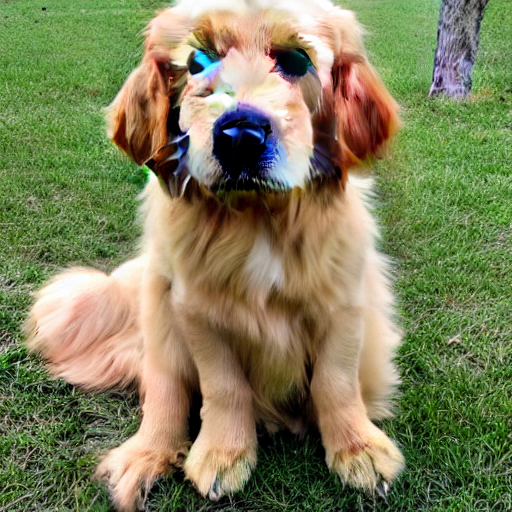
\includegraphics[width=0.3\textwidth]{golden_retriever_before.png}
    \caption{Resultado generado por el modelo preentrenado para el prompt: \textit{``a photo of a golden retriever''}.}
    \label{fig:golden-before}
\end{figure}

\paragraph{\textbf{Resultado tras la especialización del modelo}} \mbox{}\\[0.5em]
Tras aplicar la técnica de modificación del espacio latente, el modelo fue capaz de representar de forma mucho más precisa la raza solicitada. La imagen resultante muestra un perro con expresión realista, pelaje detallado, proporciones correctas y una pose reconocible. El resultado evidencia una mejora tanto estética como semántica.

\begin{figure}[H]
    \centering
    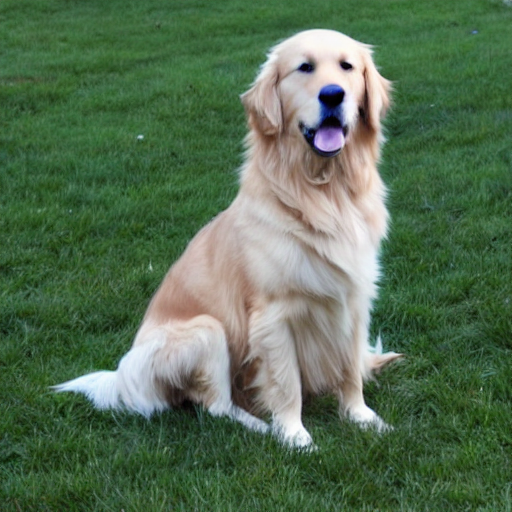
\includegraphics[width=0.3\textwidth]{golden_retriever_after.png}
    \caption{Resultado generado tras la especialización del modelo para el prompt: \textit{``a photo of a golden retriever''}.}
    \label{fig:golden-after}
\end{figure}

\subsubsection{Evaluación de coherencia semántica con CLIP}

Para respaldar cuantitativamente esta mejora, se empleó el modelo \texttt{CLIP ViT-L/14}, que permite calcular la similitud entre imágenes y texto. Se utilizó el concepto de \textit{CLIP Score relativo}, que compara la afinidad de dos imágenes frente a un mismo prompt.

\begin{table}[H]
\centering
\renewcommand{\arraystretch}{1.5}
\begin{tabular}{|p{6cm}|c|}
\hline
\rowcolor{gray!30}
\textbf{Imagen generada} & \textbf{CLIP Score relativo} \\
\hline
Modelo preentrenado & 0.0659 \\
\hline
Modelo especializado & 0.9341 \\
\hline
\end{tabular}
\caption{Similitud relativa medida con CLIP}
\label{tab:clip-golden}
\end{table}

Para facilitar la interpretación de los resultados, la Figura~\ref{fig:clip_bar} muestra una representación gráfica de los valores obtenidos. Esta visualización permite apreciar de forma más clara la diferencia de rendimiento semántico entre ambos modelos ante un mismo prompt, reflejando el impacto directo de la especialización sobre la alineación texto-imagen.

\begin{figure}[H]
    \centering
    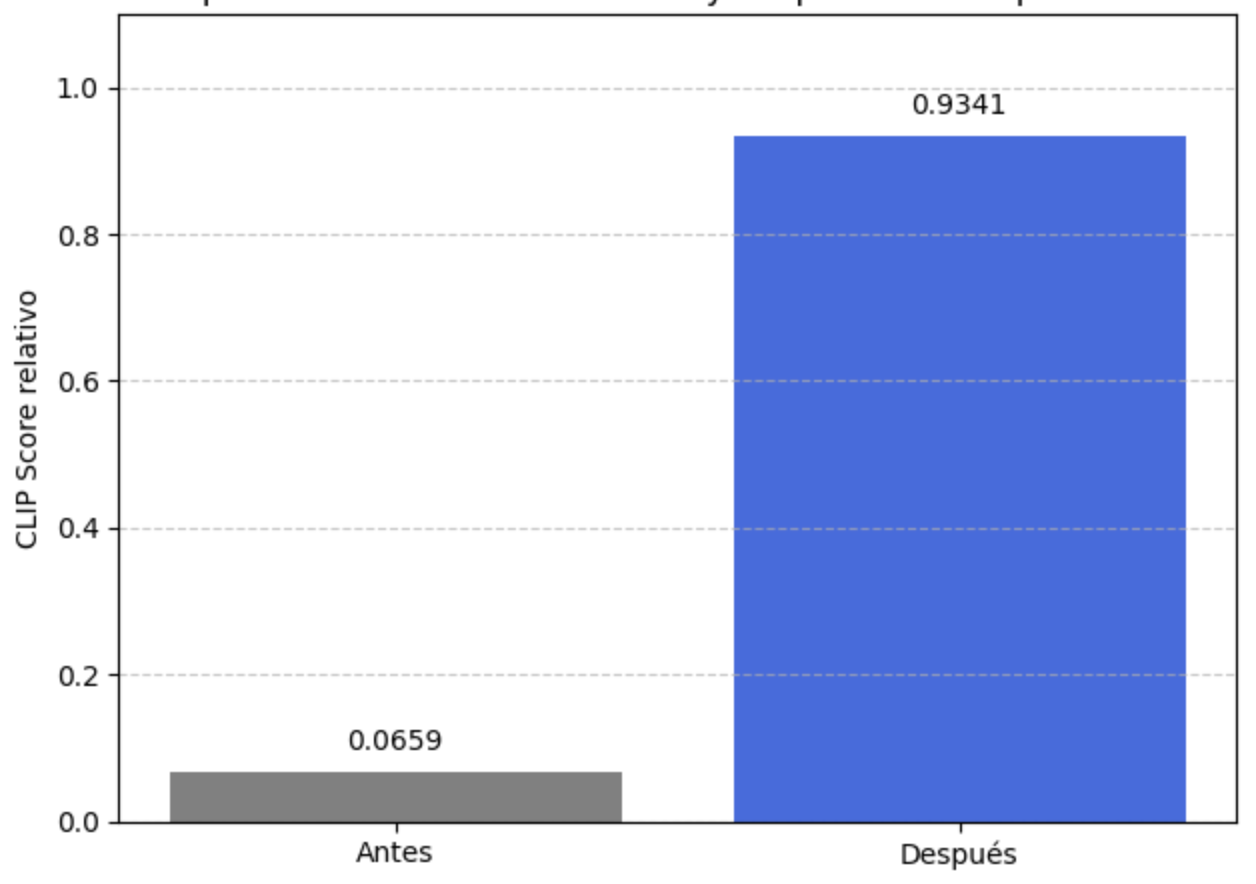
\includegraphics[width=0.4\textwidth]{clip_bar.png}
    \caption{Comparación visual del CLIP Score relativo.}
    \label{fig:clip_bar}
\end{figure}

En esta gráfica se visualiza de forma clara la mejora lograda. Mientras que el modelo original apenas logra asociar la imagen con el concepto de ``golden retriever'', el modelo especializado alcanza un nivel de coherencia semántica casi perfecto. Esto confirma que la técnica utilizada no solo mejora la calidad visual, sino también la capacidad del modelo para representar correctamente conceptos específicos.

La mejora obtenida es significativa: el modelo especializado alcanza una puntuación de similitud casi 15 veces superior a la del modelo base. Este incremento cuantitativo confirma que la adaptación del espacio latente no solo mejora la fidelidad visual, sino que también optimiza la coherencia semántica desde la perspectiva de modelos multimodales como CLIP, lo que refuerza su utilidad en tareas de búsqueda visual guiada por lenguaje.

\subsubsection{Análisis del coste de entrenamiento}

Para evaluar la viabilidad del entrenamiento personalizado, se midieron los principales factores que impactan en el coste computacional del proceso. Estos valores permiten estimar la escalabilidad del enfoque en distintos entornos de ejecución.

\begin{table}[H]
\centering
\renewcommand{\arraystretch}{1.5}
\begin{tabular}{p{5cm}p{9cm}}
\rowcolor{gray!30}
\textbf{Recurso} & \textbf{Especificaciones del servidor utilizado} \\
\rowcolor{gray!10}
Procesador & AMD Ryzen Threadripper 2920X, 12 núcleos físicos, 24 hilos, hasta 3.5 GHz \\
Memoria RAM & 62 GiB totales, disponibles: 60 GiB libres \\
\rowcolor{gray!10}
GPU & 2x NVIDIA TITAN RTX, 24 GiB de VRAM cada una \\
Sistema operativo & Ubuntu 24.04, kernel 6.8.0-59-generic, arquitectura x86\_64 \\
\rowcolor{gray!10}
CUDA y Drivers & CUDA 12.4, Driver NVIDIA 550.163.01 \\
Duración del entrenamiento & Aprox. 5 horas \\
\rowcolor{gray!10}
Tamaño del modelo entrenado & 4.0K (tamaño en disco del directorio \texttt{stable-dog-output}) \\
Frameworks utilizados & \texttt{diffusers}, \texttt{transformers}, \texttt{PyTorch}, \texttt{torchvision} \\
\rowcolor{gray!10}
Técnicas aplicadas & DreamBooth, checkpointing, half precision (float16), batch size adaptativo \\
\end{tabular}
\caption{Recursos técnicos del servidor utilizado para el entrenamiento final}
\label{tab:servidor-entrenamiento}
\end{table}

\subsubsection{Evaluación de la generalización del modelo}

Además de mejorar la generación de razas específicas como el \textit{golden retriever}, resulta clave comprobar si el modelo especializado conserva su capacidad para generar imágenes no relacionadas con el entrenamiento. Para ello, se utilizó un prompt genérico:

\begin{center}
\textit{``a man sitting on a bench in a park''}
\end{center}

La generación se realizó antes y después de aplicar la especificación para evaluar posibles pérdidas de generalidad.

\paragraph{\textbf{Antes del entrenamiento especializado}} \mbox{}\\[0.5em]
El modelo preentrenado genera una escena coherente: un hombre de espaldas sentado en un banco, con árboles bien definidos y composición equilibrada. El resultado es visualmente aceptable y semánticamente correcto.

\begin{figure}[H]
    \centering
    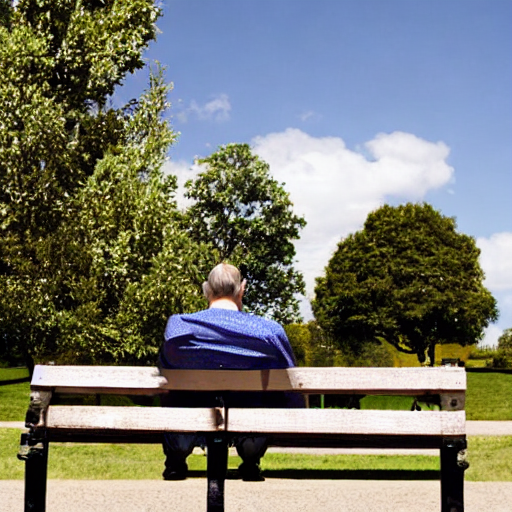
\includegraphics[width=0.4\textwidth]{man_before.png}
    \caption{Imagen generada por el modelo base con el prompt \textit{``a man sitting on a bench in a park''.}}
    \label{fig:man-before}
\end{figure}

\paragraph{\textbf{Después del entrenamiento especializado}} \mbox{}\\[0.5em]
Tras la especialización en razas de perro, el modelo mantiene su capacidad para representar correctamente conceptos no entrenados. La escena generada presenta un entorno similar, con árboles, banco y persona reconocibles, sin signos de sobreajuste. Esto sugiere que la adaptación ha sido localizada y no ha afectado negativamente a la generalización.

\begin{figure}[H]
    \centering
    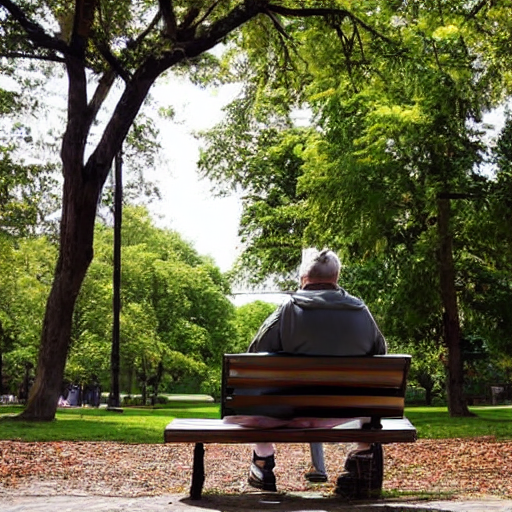
\includegraphics[width=0.4\textwidth]{man_after.png}
    \caption{Imagen generada por el modelo especializado con el mismo prompt: \textit{``a man sitting on a bench in a park''}.}
    \label{fig:man-after}
\end{figure}

\paragraph{\textbf{Conclusión}} \mbox{}\\[0.5em]
La comparación cualitativa sugiere que el modelo mantiene una buena capacidad de generalización tras la especialización. Es capaz de generar imágenes coherentes incluso para descripciones no incluidas en el entrenamiento, lo que refuerza la aplicabilidad del enfoque de DreamBooth en contextos donde es crucial preservar el conocimiento base del modelo.

\subsection{Pruebas del sistema de recuperación de imágenes}

Tras validar la generación y la calidad de las imágenes mediante el sistema desarrollado, se procedió a evaluar su uso como punto de partida para tareas de recuperación visual dentro de la plataforma JMR. El objetivo de estas pruebas fue comprobar que las imágenes generadas por el modelo podían utilizarse eficazmente como consultas en un sistema basado en similitud visual, recuperando contenidos relevantes desde una base de datos preexistente.

\subsubsection{Metodología de recuperación}

Cada prueba consistió en generar una imagen a partir de un \textit{prompt} textual y utilizarla como imagen de consulta en el sistema de recuperación implementado. Para llevar a cabo la comparación visual, se utilizaron los descriptores definidos por el estándar MPEG-7, explicados previamente en el Estado del Arte (Sección~2.3). Concretamente, se aplicaron los siguientes descriptores de color:

\begin{itemize}
    \item \textbf{Descriptor de estructura de color}, que aporta sensibilidad espacial y permite diferenciar imágenes con similares proporciones de color pero distinta disposición.
    \item \textbf{Descriptor de color escalable}, empleado en algunos casos para observar el comportamiento a distintos niveles de granularidad.
\end{itemize}

\subsubsection{Casos de prueba}

A continuación se presentan tres casos representativos en los que se utilizó una imagen generada como consulta y se evaluó el resultado de la recuperación visual, teniendo en cuenta distintas casuísticas de interacción:

\begin{itemize}
    \item \textbf{Caso 1 – Recuperación de razas de perro (Golden Retriever)}:  
    Se generó la imagen a partir del prompt \textit{``a golden retriever in the park''} y, sin visualizarla explícitamente, se utilizó directamente desde el cuadro de texto superior como imagen de consulta. El sistema recuperó imágenes de perros de aspecto y coloración similares, como se muestra en la Figura~\ref{fig:retrieval_golden}, validando la efectividad del descriptor de estructura de color para este tipo de contenido.

    \begin{figure}[H]
        \centering
        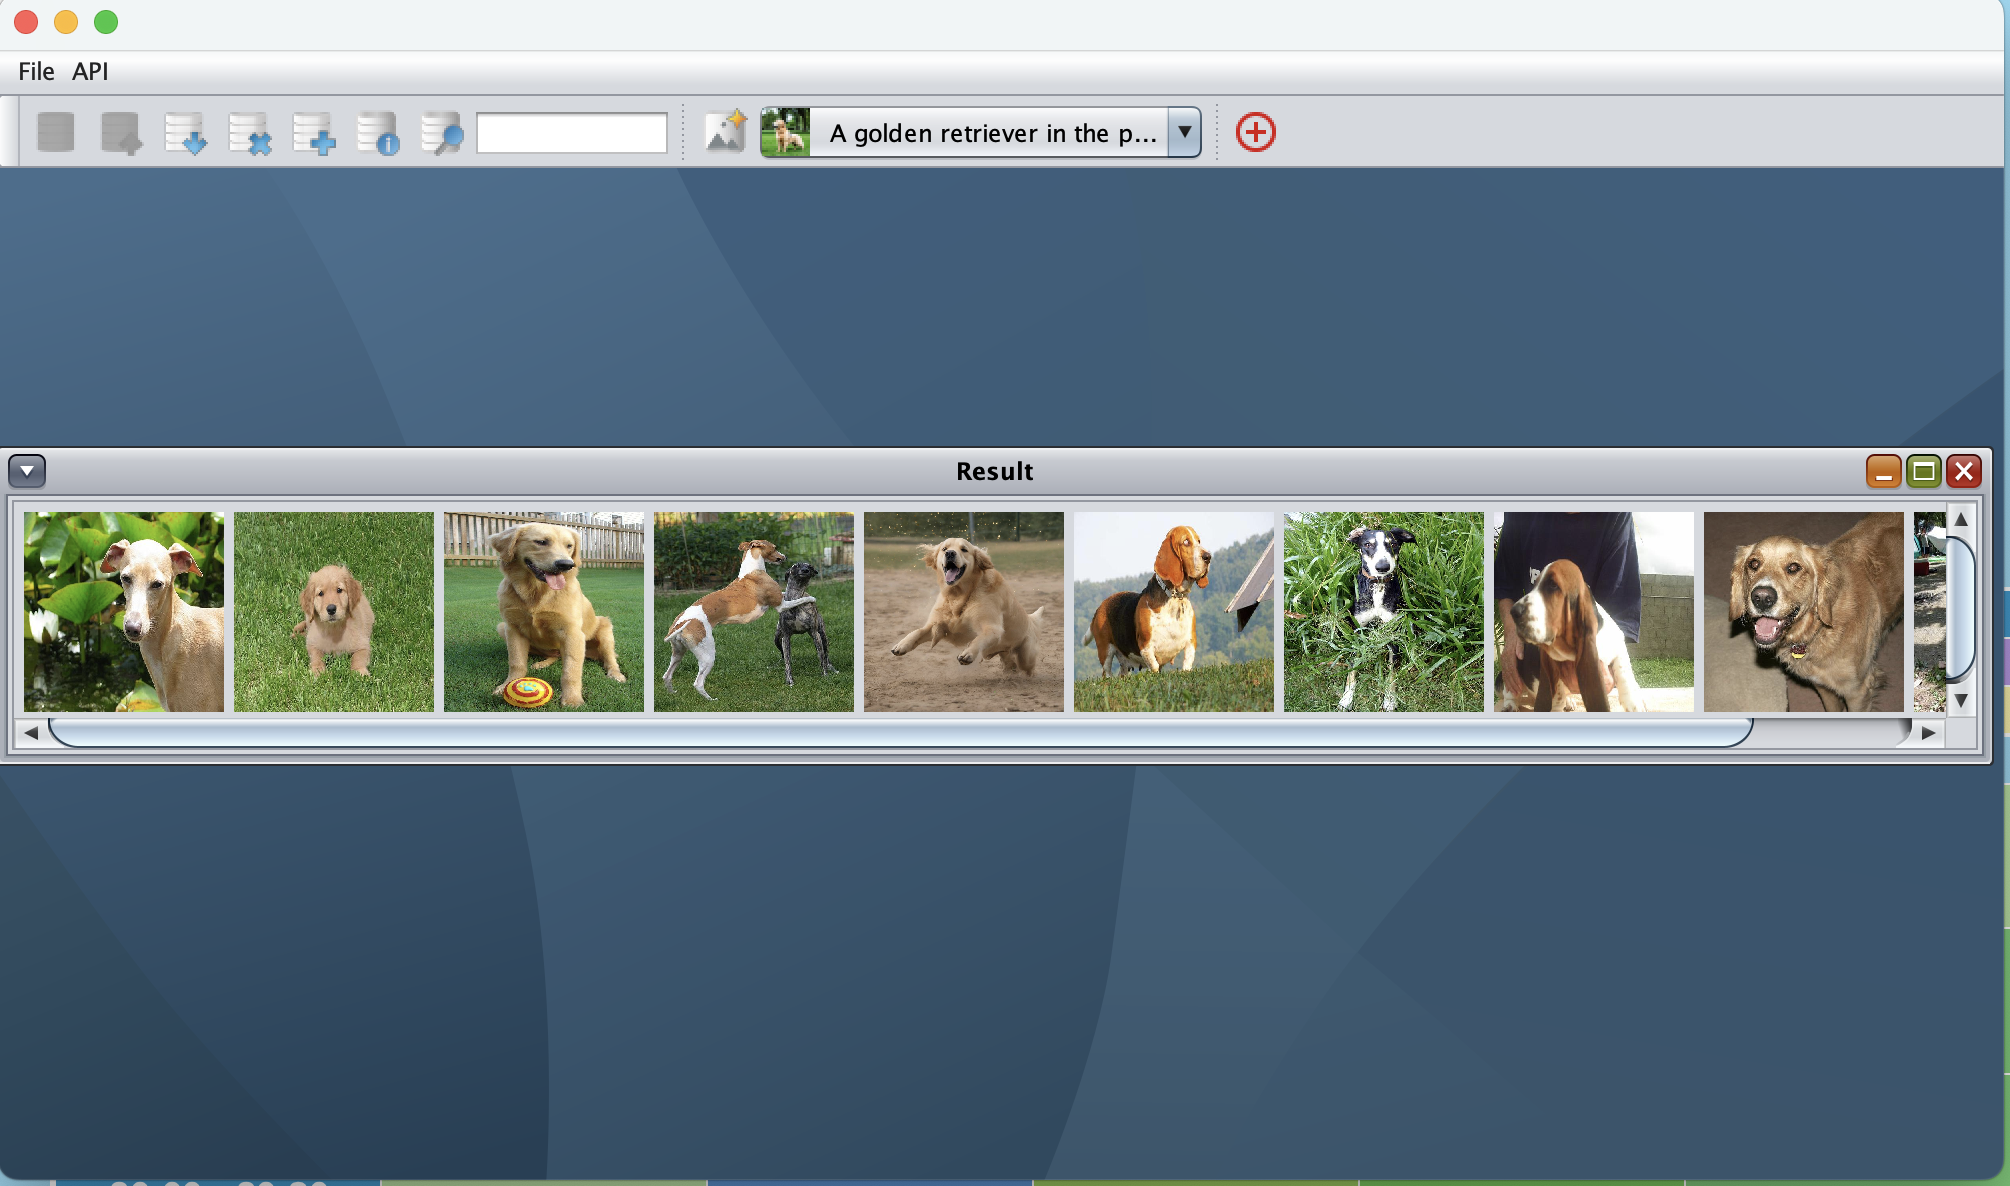
\includegraphics[width=0.7\textwidth]{pruebas/resultados_golden.png}
        \caption{Recuperación visual a partir de la imagen generada con el prompt \textit{``a golden retriever in the park''}.}
        \label{fig:retrieval_golden}
    \end{figure}

    \item \textbf{Caso 2 – Recuperación de patrones cromáticos abstractos}:  
    En este experimento se usó el prompt \textit{``a lot of colorful sprinkles''}. De forma análoga al caso anterior, la búsqueda se lanzó directamente desde el cuadro de texto superior sin abrir previamente la imagen generada. A pesar de la naturaleza abstracta de la imagen, el descriptor de estructura de color fue capaz de identificar con precisión imágenes con patrones cromáticos y distribución similares. Los resultados pueden observarse en la Figura~\ref{fig:retrieval_sprinkles}.

    \begin{figure}[H]
        \centering
        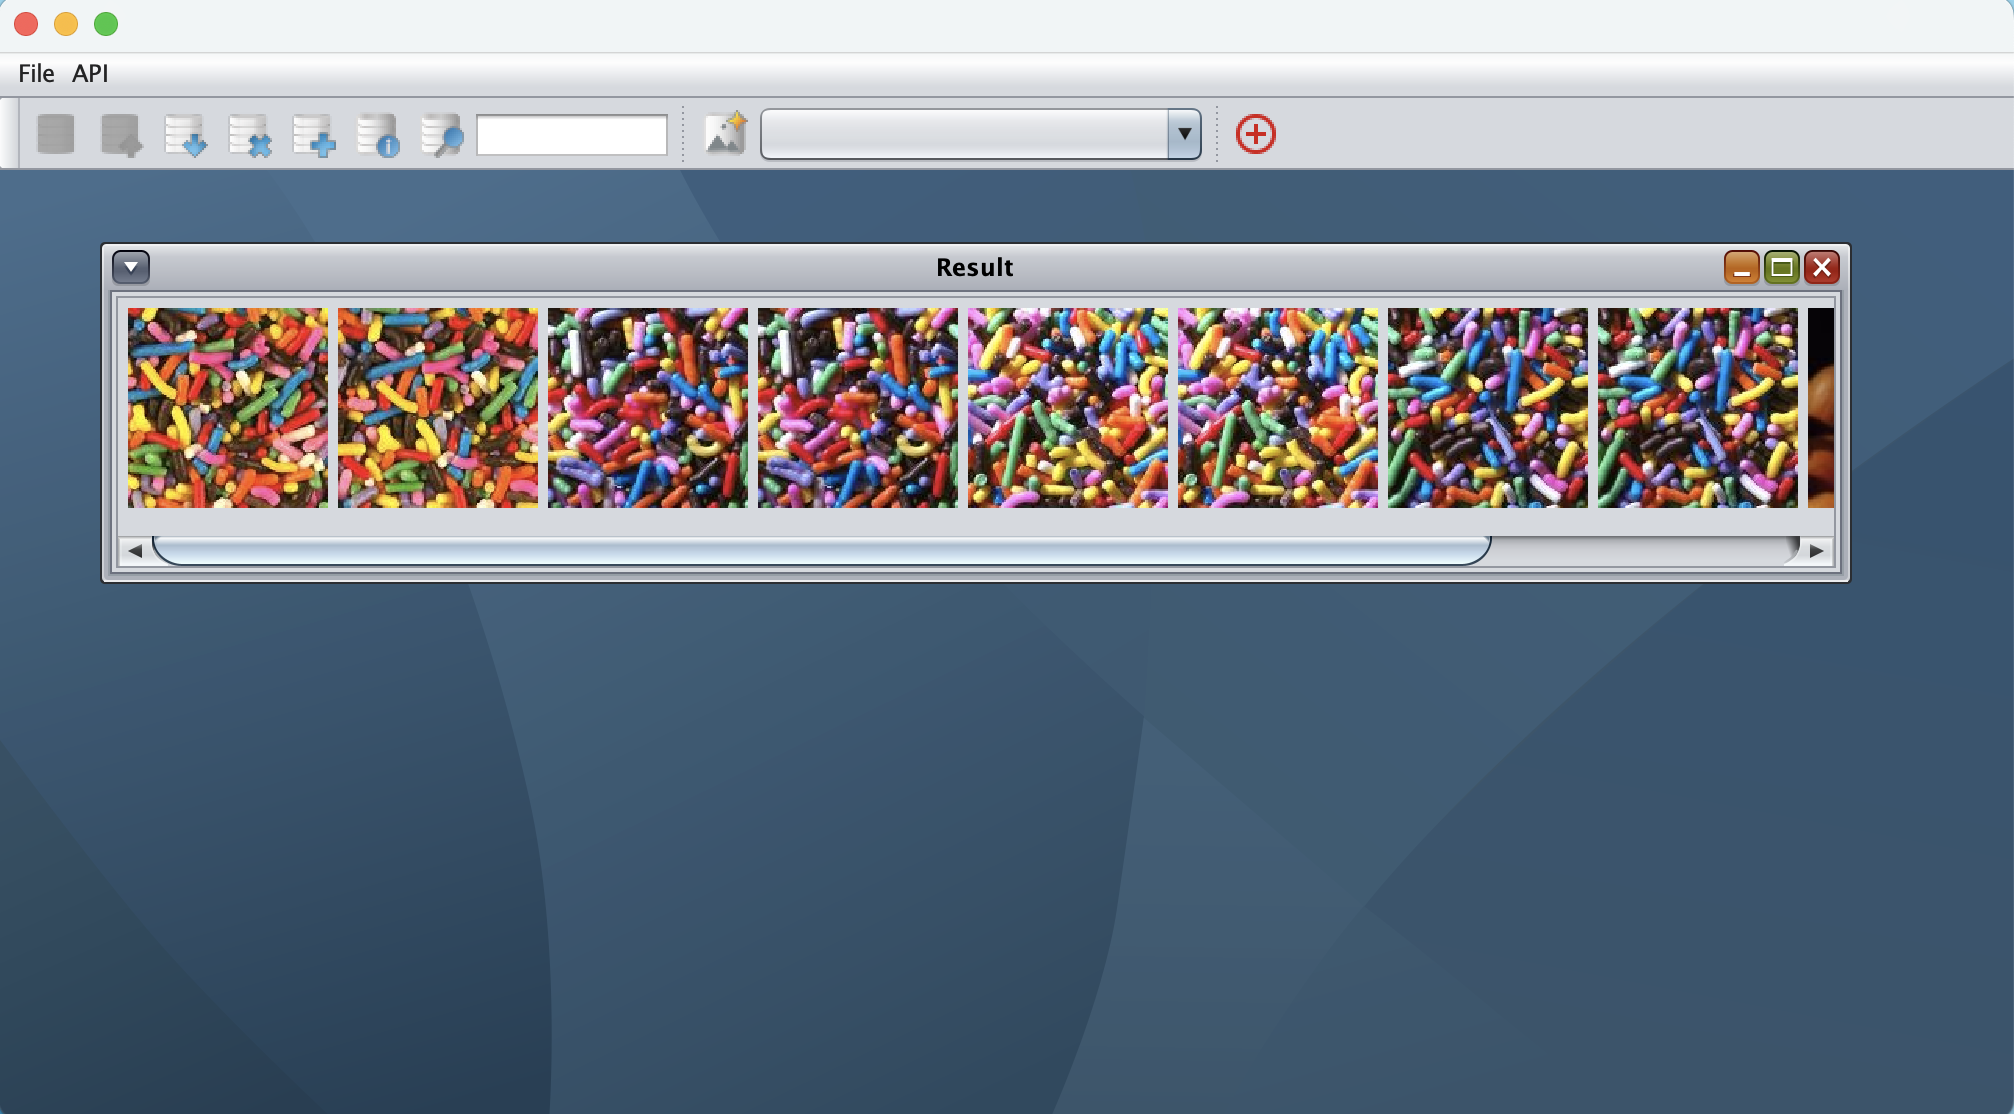
\includegraphics[width=0.7\textwidth]{pruebas/resultados.png}
        \caption{Recuperación visual a partir de la imagen generada con el prompt \textit{``a lot of colorful sprinkles''}.}
        \label{fig:retrieval_sprinkles}
    \end{figure}

    \item \textbf{Caso 3 – Recuperación de paisajes artísticos}:  
    En este caso, la imagen fue generada con el prompt \textit{``a cloudy day''} y visualizada previamente en la ventana de imagen interna. Posteriormente, se utilizó dicha imagen visualizada como entrada para la búsqueda por similitud. La Figura~\ref{fig:retrieval_cloudy} muestra los resultados, que incluyen paisajes con estructuras visuales y cromáticas similares, reflejando la sensibilidad del sistema a los tonos verdes, marrones y grises predominantes.
    \begin{figure}[H]
        \centering
        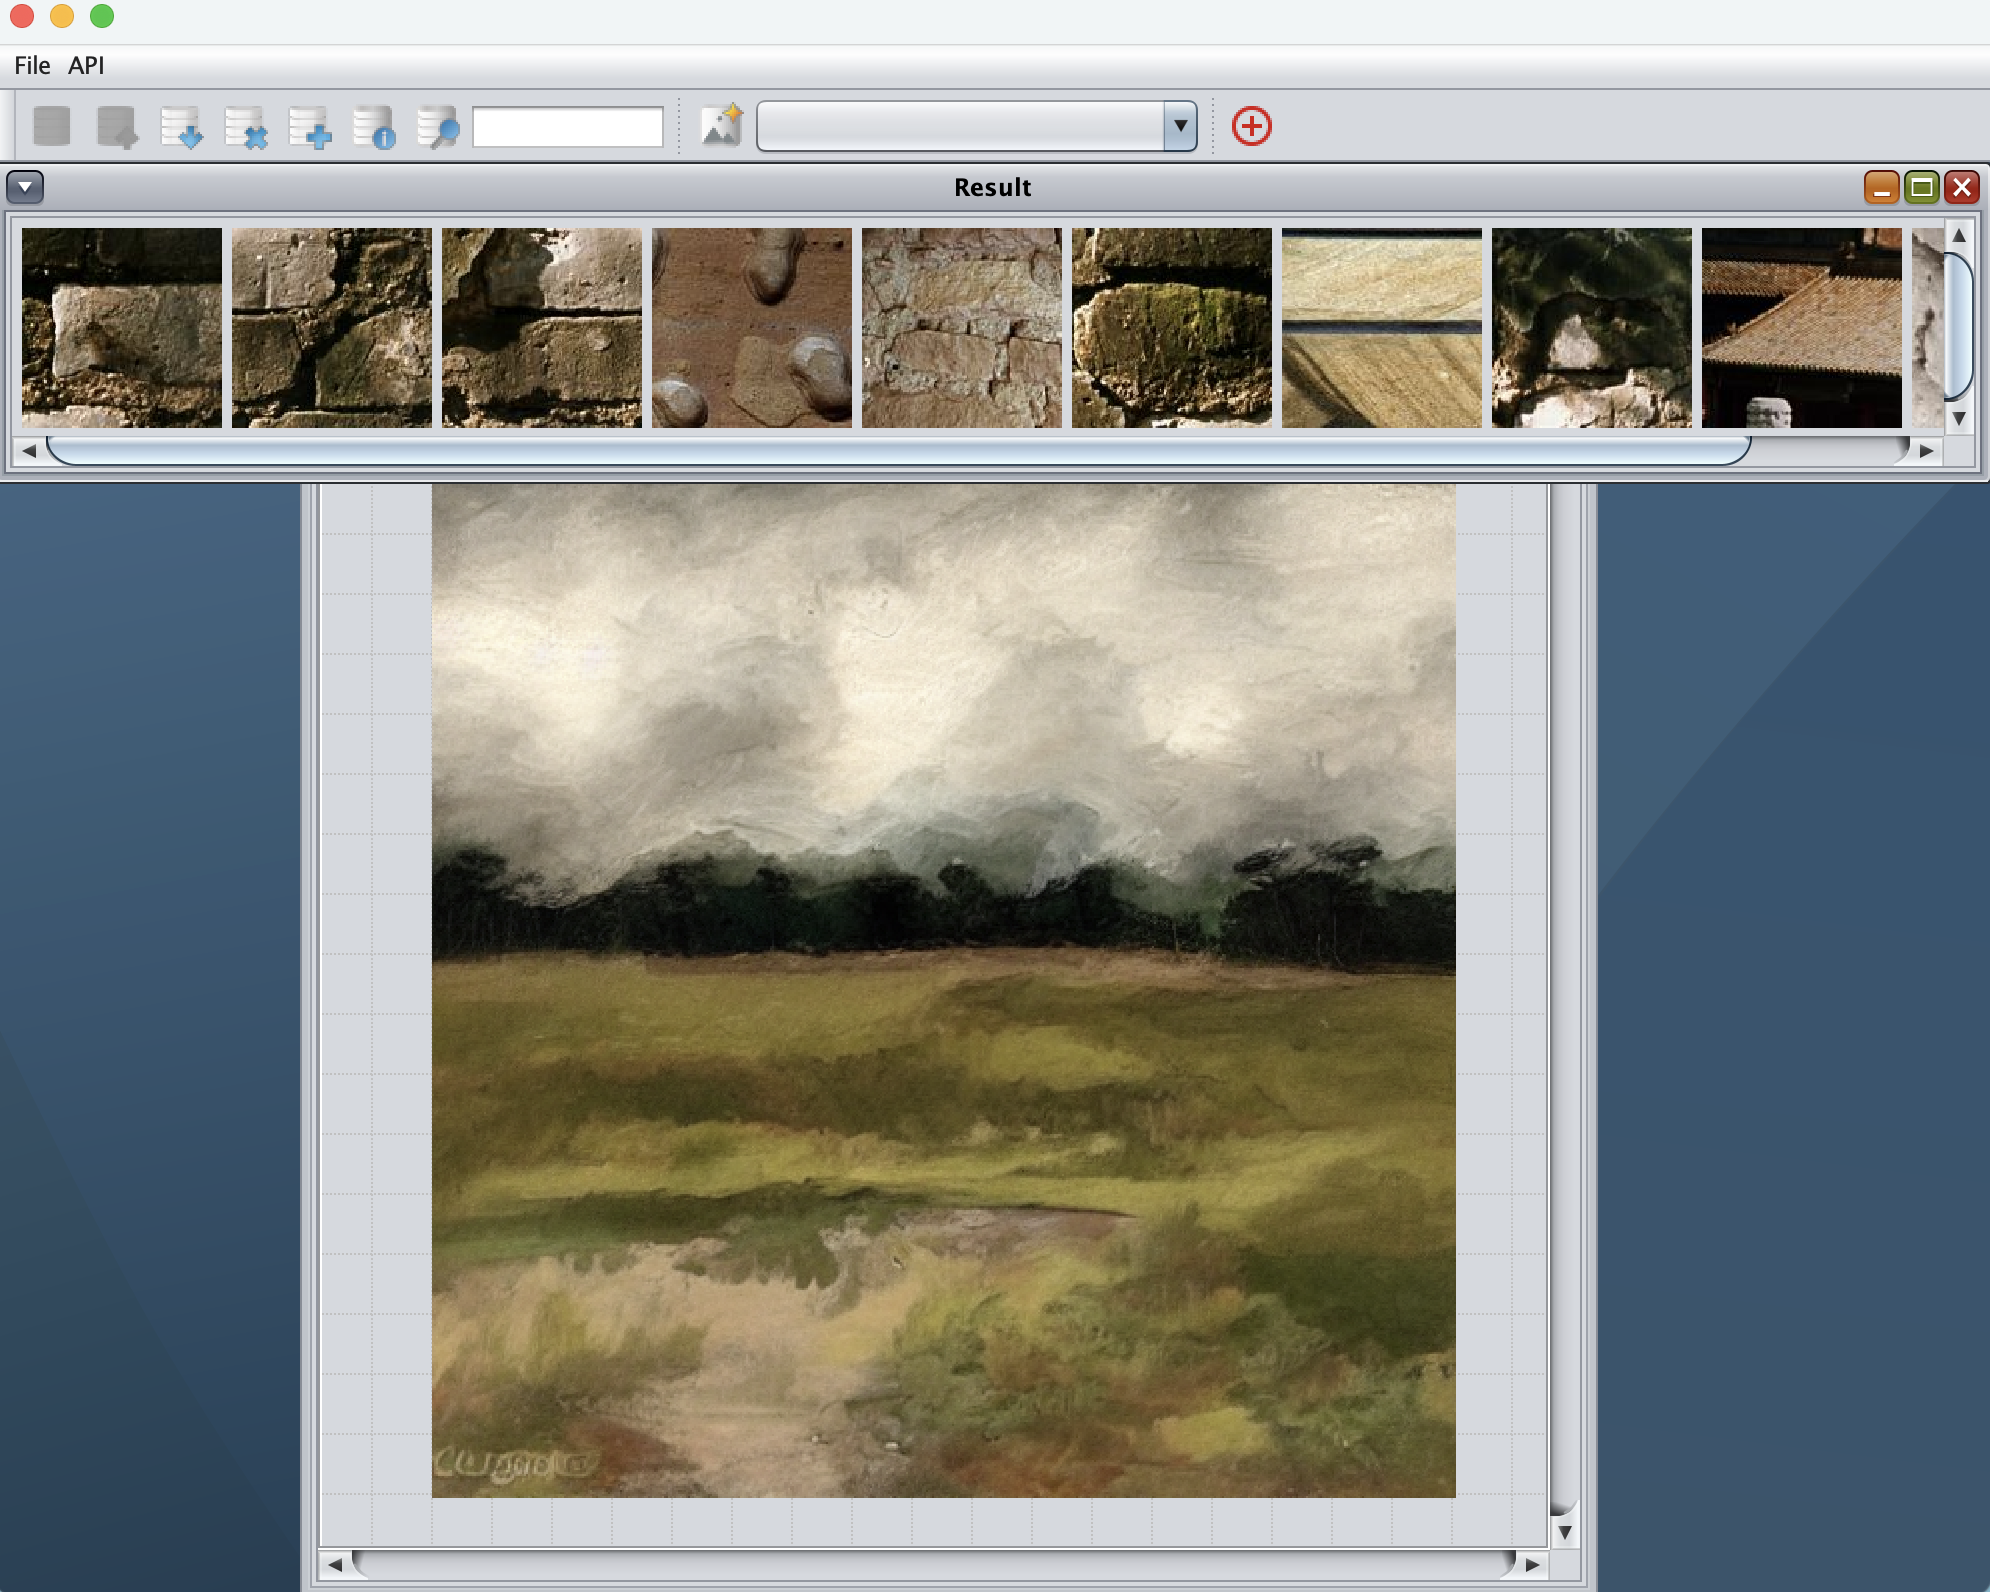
\includegraphics[width=0.7\textwidth]{pruebas/generada_resultados.png}
        \caption{Recuperación visual a partir de la imagen generada con el prompt \textit{``a cloudy day''}, tras visualizarla previamente en la aplicación.}
        \label{fig:retrieval_cloudy}
    \end{figure}

\end{itemize}

\subsubsection{Análisis de resultados}

Los casos de prueba realizados muestran un comportamiento coherente del sistema en distintos contextos de consulta. El uso de imágenes generadas como entrada ha resultado eficaz tanto en escenas estructuradas (como retratos de animales) como en patrones visuales abstractos y paisajes artísticos.

Se observó que el descriptor de estructura de color fue especialmente robusto en todos los casos, logrando identificar similitudes perceptuales relevantes incluso cuando las imágenes diferían en contenido semántico pero compartían distribuciones cromáticas o composiciones similares. En el caso del paisaje (\textit{a cloudy day}), la inclusión del descriptor de color escalable permitió una recuperación más precisa en niveles de detalle finos, especialmente al tratarse de gradientes suaves y variaciones tonales sutiles.

En cuanto a las formas de interacción, tanto la búsqueda directa desde el cuadro de texto como la reutilización tras visualizar la imagen demostraron ser funcionales. La posibilidad de lanzar consultas sin necesidad de abrir manualmente la imagen generada optimiza el flujo de trabajo, mientras que la reutilización posterior ofrece flexibilidad en casos donde se desea confirmar visualmente el contenido antes de iniciar la recuperación.

En resumen, los resultados refuerzan la idea de que el sistema no solo genera imágenes coherentes, sino que también las convierte en representaciones visuales útiles para tareas de recuperación basada en contenido, cerrando así el ciclo entre lenguaje natural, generación visual e indexación semántica.

\subsection{Conclusiones}

Los resultados obtenidos demuestran que las imágenes generadas por el sistema no solo presentan coherencia visual y semántica con los \textit{prompts} originales, sino que también son efectivas como entrada para tareas de recuperación basada en contenido visual. Esta doble funcionalidad—generación e indexación—consolida el papel del sistema como puente entre el lenguaje natural y la búsqueda visual, permitiendo transformar descripciones textuales en imágenes interpretables por algoritmos de recuperación.

En los distintos casos de estudio realizados, se ha evidenciado la versatilidad del sistema ante diversos tipos de contenido:

\begin{itemize}
    \item En el caso del \textbf{golden retriever}, la imagen generada permitió recuperar con éxito otras imágenes de perros de aspecto similar, validando la capacidad del sistema para tratar conceptos visuales bien definidos y estructurados.
    \item En la prueba con \textbf{sprinkles de colores}, se comprobó la sensibilidad del sistema a patrones cromáticos abstractos, lo que pone de manifiesto su aplicabilidad más allá de objetos concretos.
    \item En el escenario del \textbf{paisaje nublado}, la combinación de descriptores permitió capturar matices tonales y composiciones complejas, como las propias de escenas artísticas o estilizadas.
\end{itemize}

A nivel de implementación, la utilización de los descriptores visuales definidos por MPEG-7—en particular el de \textit{estructura de color} y, en menor medida, el \textit{color escalable}—resultó una elección acertada. Ambos descriptores ofrecieron un equilibrio adecuado entre coste computacional y capacidad discriminativa, permitiendo recuperar imágenes relevantes incluso en bases de datos con alta variabilidad visual.

Por otro lado, las distintas casuísticas de uso (búsqueda directa desde el cuadro de texto o reutilización tras visualización) demostraron que el sistema se adapta a diferentes flujos de trabajo, manteniendo la consistencia funcional en todos los casos.

En definitiva, se ha validado que el sistema desarrollado puede integrarse eficazmente en plataformas de recuperación visual y servir como base para futuros desarrollos donde la interacción entre texto e imagen sea fundamental. Esto abre la puerta a aplicaciones en múltiples dominios como educación, accesibilidad, archivos visuales o interfaces conversacionales basadas en imágenes generadas.
